\documentclass{beamer}
% Use DS9 global theme
\usepackage{../../../shared/templates/ds9_theme}

% Title page configuration
\title[CH22 Magnetism]{PHYS12 CH22: Magnetism}
\subtitle{Sections 22.1-22.8}
\author[Mr. Gullo]{Mr. Gullo}
\date[April 2025]{April, 2025}

\begin{document}

% Title slide
\begin{frame}
\titlepage
\end{frame}

% Learning objectives
\begin{frame}{Learning Objectives}
\begin{block}{By the end of this presentation, you should be able to:}
\begin{itemize}
\item Describe the basic properties of magnets and magnetic fields
\item Explain ferromagnetism and how electromagnets work
\item Understand magnetic field lines and their properties
\item Calculate the force on a moving charge in a magnetic field
\item Apply the right-hand rule to determine the direction of magnetic forces
\item Explain the Hall effect and its applications
\item Calculate the force on a current-carrying conductor in a magnetic field
\item Determine the torque on a current loop in a magnetic field
\end{itemize}
\end{block}
\end{frame}

% Outline slide
\begin{frame}{Outline}
\tableofcontents
\end{frame}

\section{Magnets and Magnetic Fields}

% Basic concepts of magnetism
\begin{frame}{Basic Concepts of Magnetism}
\begin{block}{Magnetism}
Properties of magnets, effect of magnetic force on moving charges and currents, and creation of magnetic fields by currents.
\end{block}

\begin{columns}
\column{0.6\textwidth}
\begin{itemize}
\item Two types of magnetic poles:
  \begin{itemize}
  \item North magnetic pole
  \item South magnetic pole
  \end{itemize}
\item North magnetic poles are attracted toward Earth's geographic north pole
\item Like poles repel, unlike poles attract
\item Magnetic poles always occur in pairs—cannot be isolated
\end{itemize}

\column{0.4\textwidth}
\begin{figure}
    \centering
    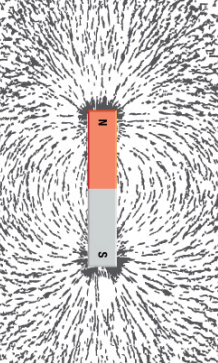
\includegraphics[width=1\linewidth]{phys12-magnetism-magnetic-field-generator.png}
\end{figure}
\end{columns}
\end{frame}

% Ferromagnets and Electromagnets
\begin{frame}{Ferromagnets and Electromagnets}
\begin{columns}
\column{0.5\textwidth}
\textbf{Ferromagnetic Materials}
\begin{itemize}
\item Materials exhibiting strong magnetic effects (e.g., iron)
\item Atoms act like small magnets (due to internal currents)
\item Form millimeter-sized regions called \textbf{domains}
\item Domains can align to create permanent magnets
\item Above Curie temperature, thermal agitation destroys alignment
\end{itemize}

\column{0.5\textwidth}
\textbf{Electromagnets}
\begin{itemize}
\item Use electric currents to make magnetic fields
\item Often aided by induced fields in ferromagnetic materials
\item Field strength depends on current and number of turns
\item Field can be turned on and off
\end{itemize}
\end{columns}

\end{frame}

% Magnetic field lines
\begin{frame}{Magnetic Field Lines}
\begin{block}{Magnetic Field Representation}
Magnetic fields can be pictorially represented by magnetic field lines.
\end{block}

\begin{columns}
\column{0.6\textwidth}
\textbf{Properties of magnetic field lines:}
\begin{enumerate}
\item The field is tangent to the magnetic field line
\item Field strength is proportional to line density
\item Field lines cannot cross
\item Field lines are continuous loops
\end{enumerate}

\column{0.4\textwidth}
\begin{figure}
    \centering
    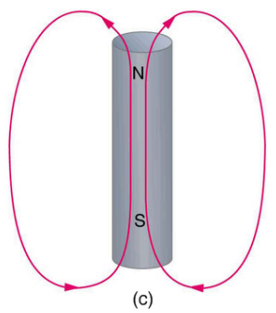
\includegraphics[width=1\linewidth]{phys12-magnetism-magnetic-force-on-wire.png}
\end{figure}
\end{columns}
\end{frame}

\section{Magnetic Forces on Charges and Currents}

% Force on moving charge
\begin{frame}{Force on Moving Charge in Magnetic Field}
\begin{block}{Magnetic Force Formula}
The magnitude of the magnetic force on a moving charge $q$ is:
\begin{equation}
F = qvB\sin\theta
\end{equation}
where $\theta$ is the angle between the directions of $\vec{v}$ and $\vec{B}$.
\end{block}

\begin{columns}
\column{0.5\textwidth}
\begin{itemize}
\item SI unit for magnetic field $B$: tesla (T)
\item $1 \text{ T} = \frac{1 \text{ N}}{\text{A}\cdot\text{m/s}} = \frac{1 \text{ N}}{\text{A}\cdot\text{m}}$
\item Force direction given by right hand rule 1 (RHR-1)
\item Force is perpendicular to plane formed by $\vec{v}$ and $\vec{B}$
\item Force is zero if $\vec{v}$ is parallel to $\vec{B}$
\end{itemize}

\column{0.5\textwidth}
\begin{figure}
    \centering
    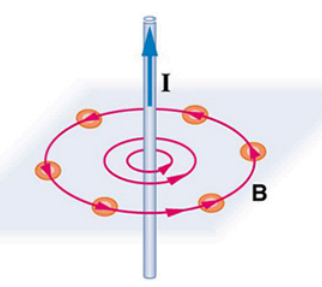
\includegraphics[width=0.75\linewidth]{phys12-magnetism-magnetic-field-lines-generator.png}
\end{figure}
\end{columns}
\end{frame}


\begin{frame}{Force on Moving Charge in Magnetic Field}
    \begin{figure}
        \centering
        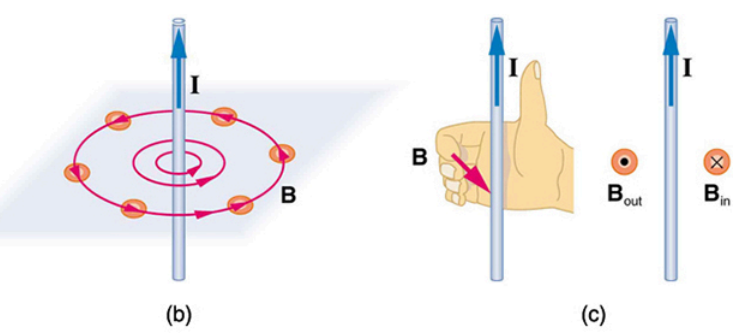
\includegraphics[width=0.75\linewidth]{phys12-magnetism-right-hand-rule-force.png}
    \end{figure}
\end{frame}
\begin{frame}{Force on Moving Charge in Magnetic Field}
    
\begin{figure}
    \centering
    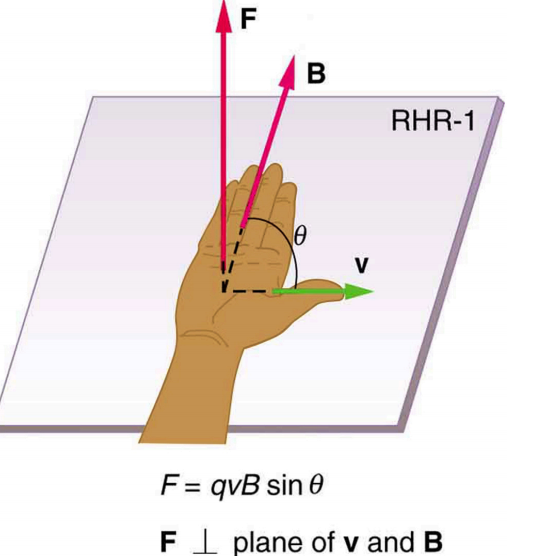
\includegraphics[width=1\linewidth]{phys12-magnetism-right-hand-rule-current.png}
\end{figure}
\end{frame}

% Applications of force on moving charge
\begin{frame}{Applications of Force on Moving Charges}
\begin{block}{Circular Motion in Magnetic Field}
Magnetic force can supply centripetal force causing charged particles to move in circular paths with radius:
\begin{equation}
r = \frac{mv}{qB}
\end{equation}
where $v$ is the component of velocity perpendicular to $\vec{B}$.
\end{block}

\begin{columns}
\column{0.6\textwidth}
\begin{itemize}
\item Basis for many applications:
  \begin{itemize}
  \item Mass spectrometers
  \item Cyclotrons
  \item Synchrotrons
  \item Particle detectors
  \end{itemize}
\item Only affects moving charges
\item Direction changes with charge polarity
\end{itemize}

\column{0.4\textwidth}
\begin{figure}
    \centering
    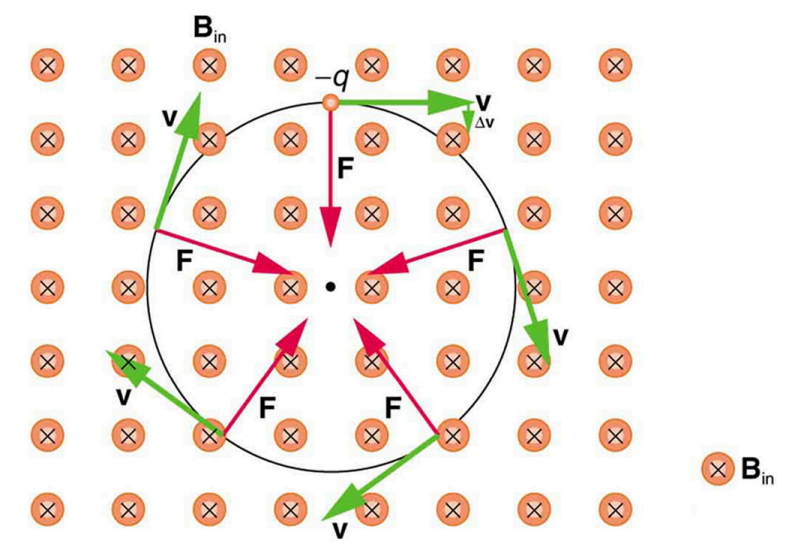
\includegraphics[width=1\linewidth]{phys12-magnetism-magnetic-force-on-current-loop.png}
\end{figure}
\end{columns}
\end{frame}

% Hall Effect
\begin{frame}{The Hall Effect}
\begin{block}{Hall Effect Definition}
The creation of voltage $\varepsilon$ (Hall emf) across a current-carrying conductor by a magnetic field.
\end{block}

\begin{columns}
\column{0.5\textwidth}
\begin{itemize}
\item Hall emf is given by:
\begin{equation}
\varepsilon = Blv
\end{equation}
\item $B$, $l$, and $v$ must be mutually perpendicular
\item For conductor of width $l$ with charges moving at speed $v$
\item Applications:
  \begin{itemize}
  \item Measuring magnetic fields
  \item Determining charge carrier type and density
  \item Hall effect sensors
  \end{itemize}
\end{itemize}

\column{0.5\textwidth}
\begin{figure}
    \centering
    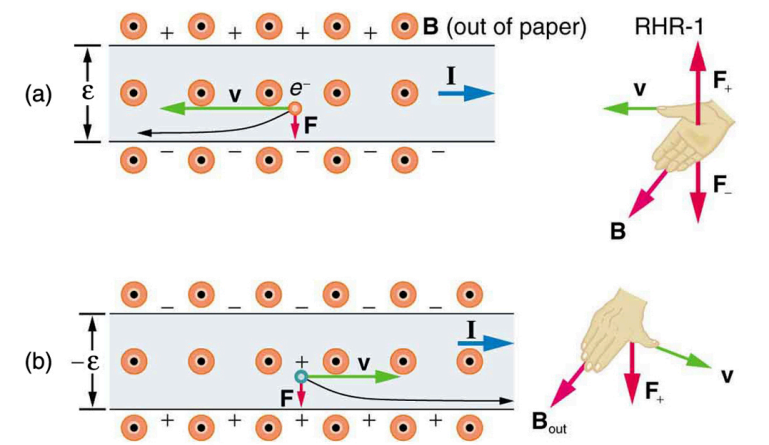
\includegraphics[width=1\linewidth]{phys12-magnetism-hall-effect.png}
\end{figure}
\end{columns}
\end{frame}

% Force on current-carrying conductor
\begin{frame}{Magnetic Force on a Current-Carrying Conductor}
\begin{block}{Force Formula}
The magnetic force on a current-carrying conductor is:
\begin{equation}
F = IlB\sin\theta
\end{equation}
where $I$ is the current, $l$ is the length of the conductor, $B$ is the magnetic field strength, and $\theta$ is the angle between $\vec{I}$ and $\vec{B}$.
\end{block}


\begin{itemize}
\item Direction follows RHR-1 with thumb in direction of $\vec{I}$
\item Maximum force when conductor is perpendicular to field
\item No force when conductor is parallel to field
\item Basis for electric motors
\end{itemize}


\end{frame}

% Torque on current loop
\begin{frame}{Torque on a Current Loop: Motors and Meters}
\begin{block}{Torque Formula}
The torque on a current-carrying loop in a uniform magnetic field is:
\begin{equation}
\tau = NIAB\sin\theta
\end{equation}
where $N$ is the number of turns, $I$ is the current, $A$ is the loop area, $B$ is the magnetic field strength, and $\theta$ is the angle between the perpendicular to the loop and the magnetic field.
\end{block}

\begin{columns}
\column{0.5\textwidth}
\begin{itemize}
\item Maximum torque when loop is parallel to field
\item Zero torque when loop is perpendicular to field
\item Applications:
  \begin{itemize}
  \item Electric motors
  \item Galvanometers
  \item Ammeters
  \item Voltmeters
  \end{itemize}
\end{itemize}

\column{0.5\textwidth}
\begin{figure}
    \centering
    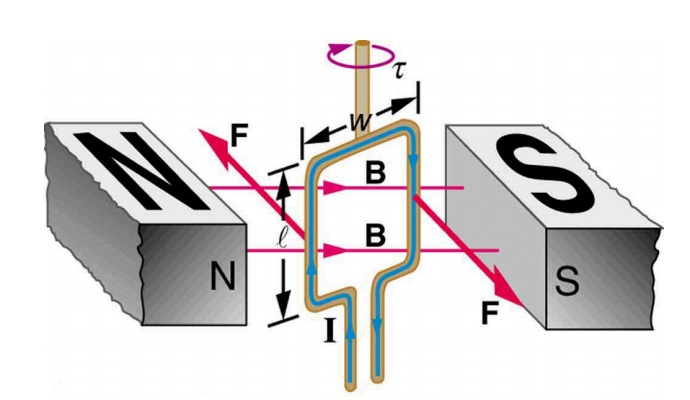
\includegraphics[width=0.9\linewidth]{phys12-magnetism-torque-on-current-loop.png}
\end{figure}
\end{columns}
\end{frame}

\section{Example Problems}

% I do example
\begin{frame}{Example 1: "I do"}
\begin{block}{Problem}
Calculate the force on an electron moving at $5.0 \times 10^6$ m/s perpendicular to a magnetic field of 0.50 T.
\end{block}
\pause
\begin{block}{Solution}
Given:
\begin{itemize}
\item Charge of electron: $q = -1.60 \times 10^{-19}$ C
\item Velocity: $v = 5.0 \times 10^6$ m/s
\item Magnetic field: $B = 0.50$ T
\item Angle: $\theta = 90°$ (perpendicular)
\end{itemize}

The negative sign indicates the force is in the direction opposite to that given by RHR-1 for a positive charge.
\end{block}
\end{frame}

\begin{frame}{Example 1: "I do"}

\begin{block}{Solution}
Given:
\begin{itemize}
\item Charge of electron: $q = -1.60 \times 10^{-19}$ C
\item Velocity: $v = 5.0 \times 10^6$ m/s
\item Magnetic field: $B = 0.50$ T
\item Angle: $\theta = 90°$ (perpendicular)
\end{itemize}

Using the formula $F = qvB\sin\theta$:

\pause

\begin{align}
F &= (-1.60 \times 10^{-19} \text{ C})(5.0 \times 10^6 \text{ m/s})(0.50 \text{ T})(\sin 90°) \\
F &= (-1.60 \times 10^{-19})(5.0 \times 10^6)(0.50)(1) \\
F &= -4.0 \times 10^{-13} \text{ N}
\end{align}

The negative sign indicates the force is in the direction opposite to that given by RHR-1 for a positive charge.
\end{block}
\end{frame}

% We do example
\begin{frame}{Example 2: "We do"}
\begin{block}{Problem}
Find the radius of the circular path of a proton with speed $3.0 \times 10^6$ m/s in a magnetic field of 0.75 T when the proton velocity is perpendicular to the field.
\end{block}
\pause

\begin{block}{Solution}
Given:
\begin{itemize}
\item Mass of proton: $m = 1.67 \times 10^{-27}$ kg
\item Charge of proton: $q = 1.60 \times 10^{-19}$ C
\item Velocity: $v = 3.0 \times 10^6$ m/s
\item Magnetic field: $B = 0.75$ T
\end{itemize}

\end{block}
\end{frame}
\begin{frame}{Example 2: "We do"}
\pause
\begin{block}{Solution}
Given:
\begin{itemize}
\item Mass of proton: $m = 1.67 \times 10^{-27}$ kg
\item Charge of proton: $q = 1.60 \times 10^{-19}$ C
\item Velocity: $v = 3.0 \times 10^6$ m/s
\item Magnetic field: $B = 0.75$ T
\end{itemize}

Using the formula $r = \frac{mv}{qB}$:

\pause

\begin{align}
r &= \frac{(1.67 \times 10^{-27} \text{ kg})(3.0 \times 10^6 \text{ m/s})}{(1.60 \times 10^{-19} \text{ C})(0.75 \text{ T})} \\
r &= \frac{5.01 \times 10^{-21}}{1.20 \times 10^{-19}} \\
r &= 4.2 \times 10^{-2} \text{ m} = 4.2 \text{ cm}
\end{align}
\end{block}
\end{frame}


% You do example
\begin{frame}{Example 3: "You do"}
\begin{block}{Problem}
A straight wire carrying a 5.0 A current is placed in a uniform magnetic field of 0.25 T. If the wire is 10 cm long and makes an angle of 30° with the field, what is the magnetic force on the wire?
\end{block}
\pause
\begin{block}{Hints}
\begin{itemize}
\item Use the formula $F = IlB\sin\theta$
\item Convert all units to SI
\item Remember to calculate the sine of the angle
\end{itemize}
\end{block}
\pause
\begin{block}{Answer (to check your work)}
$F = 0.125$ N
\end{block}
\end{frame}

% Key Equations summary
\begin{frame}{Key Equations}
\begin{block}{Magnetic Forces}
\begin{align}
F &= qvB\sin\theta & \text{(Force on moving charge)} \\
r &= \frac{mv}{qB} & \text{(Radius of circular path)} \\
\varepsilon &= Blv & \text{(Hall emf)} \\
F &= IlB\sin\theta & \text{(Force on current-carrying conductor)} \\
\tau &= NIAB\sin\theta & \text{(Torque on current loop)}
\end{align}
\end{block}

\begin{block}{Right-Hand Rules}
\begin{itemize}
\item RHR-1 for force direction: thumb in direction of $\vec{v}$ (or $\vec{I}$), fingers in direction of $\vec{B}$, palm indicates force direction
\end{itemize}
\end{block}
\end{frame}

% Summary
\begin{frame}{Summary}
\begin{itemize}
\item Magnets have north and south poles; like poles repel, unlike poles attract
\item Magnetic poles always come in pairs and cannot be isolated
\item All magnetism is created by electric current
\item Ferromagnetic materials contain domains of aligned atomic magnets
\item Magnetic fields are represented by field lines with specific properties
\item Magnetic forces act on moving charges and current-carrying conductors
\item The Hall effect creates voltage across a current-carrying conductor in a magnetic field
\item Torque on current loops in magnetic fields is the basis for motors and meters
\end{itemize}

\begin{block}{Applications}
Electromagnets, electric motors, generators, particle accelerators, mass spectrometers, Hall effect sensors, magnetic resonance imaging (MRI)
\end{block}
\end{frame}

% References slide
\begin{frame}{References}
\begin{block}{Textbook}
OpenStax Physics, Chapter 22: Magnetism, Sections 22.1-22.8
\end{block}
\end{frame}

\end{document}